\section{COMPONENT CODE GENERATOR FEATURES}

In this section will be describe the main features of the code generator, such
as the inheritance, notification channels, a standalone generator, code
regeneration strategies.

\subsection{A Stand-alone Generator}
The component code generator was designed to be a standalone application,
this means, can be executed in any O.S. as a Java Program, JAR Package or
Eclipse Plugin outside of EMF or Eclipse EMF project.\\
\\
The generator supports three ways to be a standalone :
\begin{itemize}
  \item JAR Package : The binary files are packaged in a JAR Java file using
  Ant or Eclipse Ant.
  \item Eclipse Plugin : A simple Eclipse plugin as a Jar file.
  \item Command Line : A Java command line program.
\end{itemize}
Also, the generator contains all the packages to be executed without EMF and 
can be imported to other environments running Java.

All the binarys can be dowloaded, for this, see the `Project Paths` in this
document.

\subsection{Basic Component Modeling}

The basic component model contains a at least a Container and a Component
class also a IDL struct or enumeration class.

\begin{figure*}[h!t]
\begin{center}
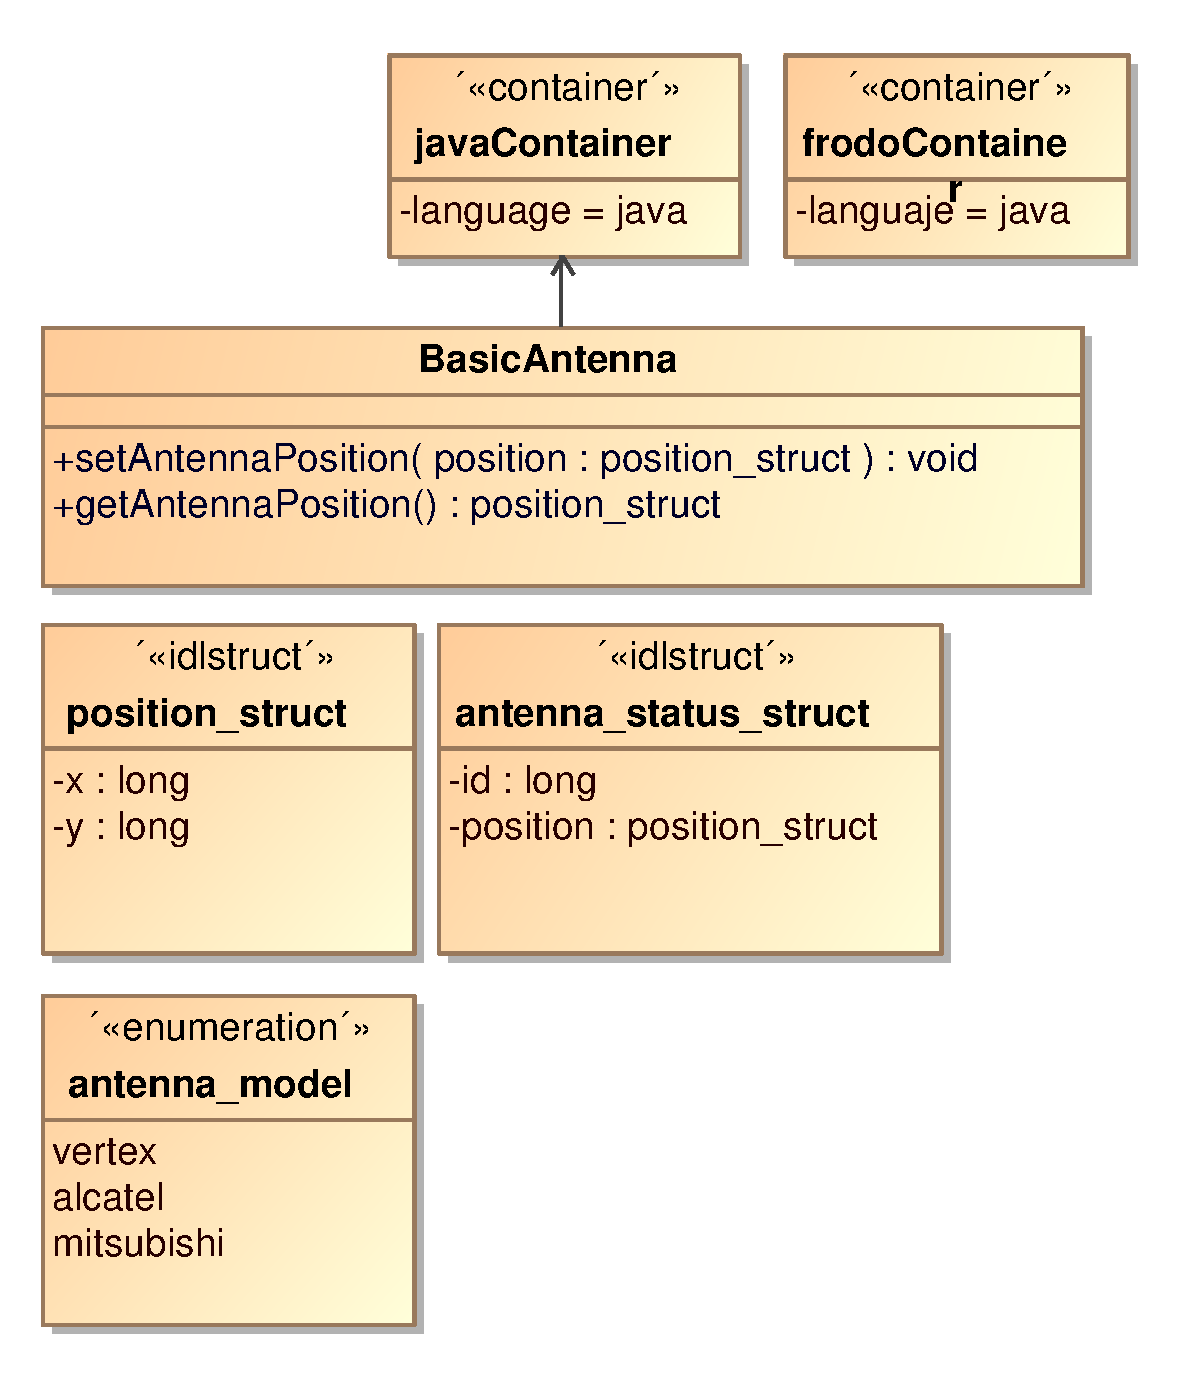
\includegraphics[scale=0.36]{images/example1}
\caption{\label{fig:vs_diag}Basic Model Definition}
\end{center}
\end{figure*} 

This example can be downloaded from:
http://acsccg.googlecode.com/files/example1.tar.gz

\subsubsection{Container Definition}
Every model should have defined at least one container. This is defined by the
stereotype  \verb+<<container>>+ and the class must have defined a property
called  `language`, the value of this property is the programming language that
the container will support (cpp, java, python).
All the containers defined are generated in the CDB configuration in the
generated code.

\begin{figure*}[h!t]
\begin{center}
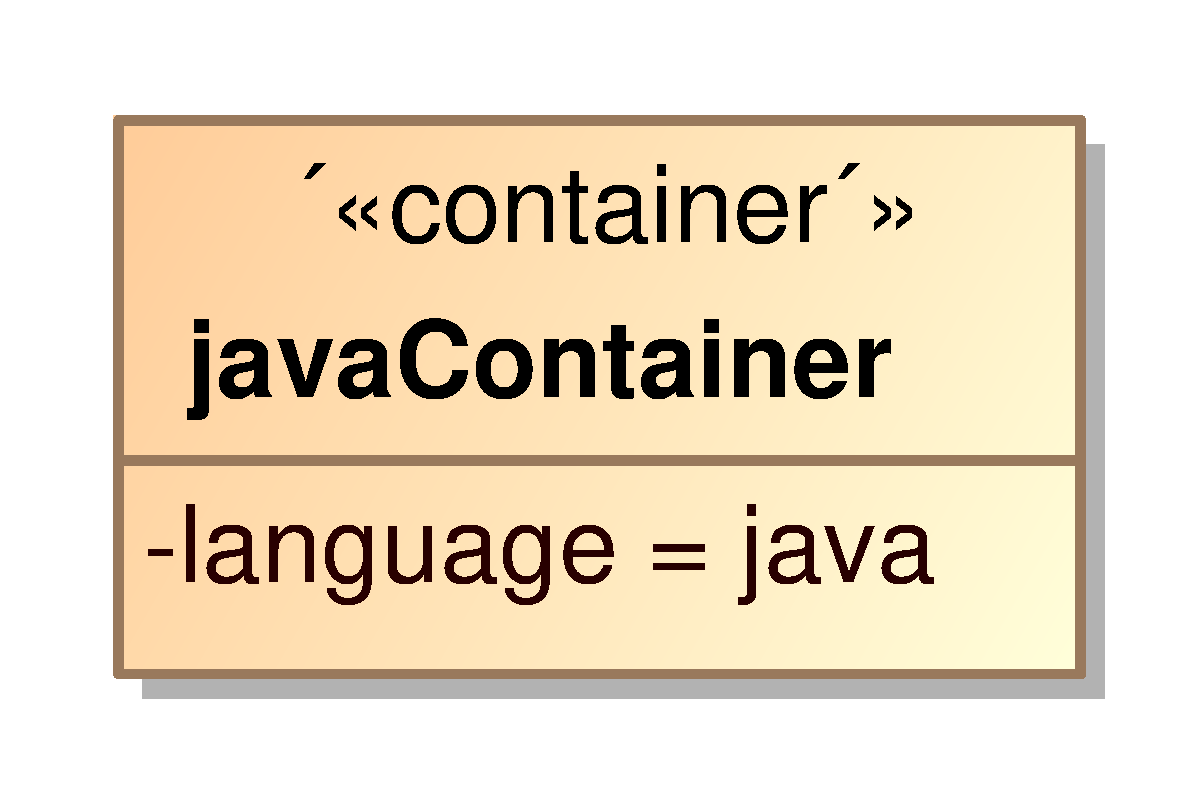
\includegraphics[scale=0.18]{images/container}
\caption{\label{fig:vs_diag}Container Definition}
\end{center}
\end{figure*} 

In the example above, the class \verb+javaContainer+ has the stereotype
\verb+<<container>>+ and the languaje for this container is \verb+java+.
Below, is the code generated for the containers, in this case the
\verb+javaContainer+.
\begin{center}
\begin{verbatim}
test/
`-- CDB
    `-- MACI
        |-- Components
        |   `-- Components.xml
        |-- Containers
        |   `-- javaContainer
        |       `-- javaContainer.xml
        `-- Managers
            `-- Manager
                `-- Manager.xml
\end{verbatim}
\end{center}

And the \verb+javaContainer.xml+ code:
\begin{center}
\begin{verbatim}
<?xml version="1.0" encoding="ISO-8859-1"?>
<Container 
    xmlns:xsi="http://www.w3.org/2001/XMLSchema-instance" 
    xmlns="urn:schemas-cosylab-com:Container:1.0" 
    xmlns:log="urn:schemas-cosylab-com:LoggingConfig:1.0" 
    ImplLang="java"
    >
    <Autoload>
     </Autoload>
     <LoggingConfig>
        <log:_ Name="jacorb@javaContainer" 
        minLogLevel="5" 
        minLogLevelLocal="5"/>
    </LoggingConfig>
</Container>
\end{verbatim}
\end{center}

\subsubsection{Component Definition}
Every class without a stereotype, the generator will recognize the class as a
component. Every class must be related to a container class, if the class is not
related to a container, the generator will not config the component in the CDB.
All component classes that are related to a container the generator will
generate:
\begin{itemize}
	\item The source component Java code (with his methods).
	\item The source java helper class.
	\item The IDL interface (with component methods).
	\item The CDB configuration for the component.
	\item The Makefile is generated with all IDL interfaces which represents each
	class component in the model.
\end{itemize}

 \begin{figure*}[h!t]
\begin{center}
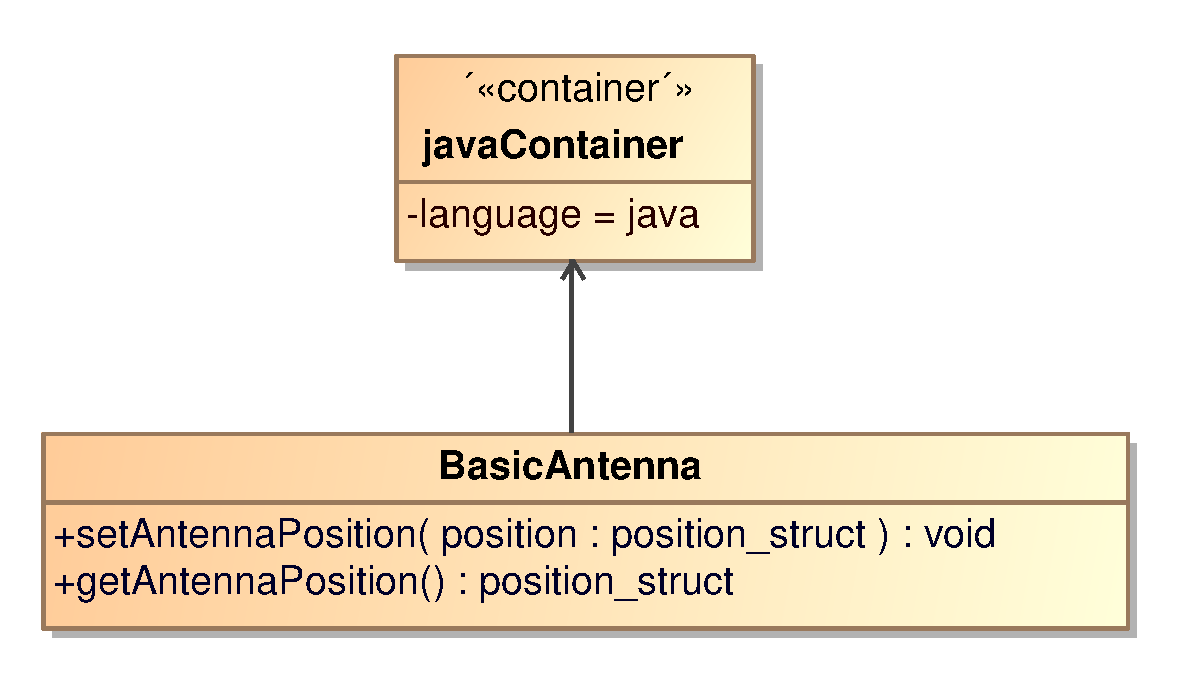
\includegraphics[scale=0.4]{images/basiccomponent}
\caption{\label{fig:vs_diag}Basic Component Definition}
\end{center}
\end{figure*} 

In the example above the class  \verb+BasicAntenna+ is a ACS component and is
related to the  \verb+javaContainer+ the name of the Java classes are prefixed
by `Base` also the IDL interfaces generated are prefixed by `Base` and example
of this the \verb+BasicAntenna+ class is generated as
\verb+BasicAntennaBase.java+ class.

\subsubsection{IDL Structs Definition}

The IDL structs are defined in a class with the stereotype \verb+<<idlstruct>>+.
In the example below the class \verb+<<antenna_status_struct>>+ has two property
that the generator will implement.

\begin{figure*}[h!t]
\begin{center}
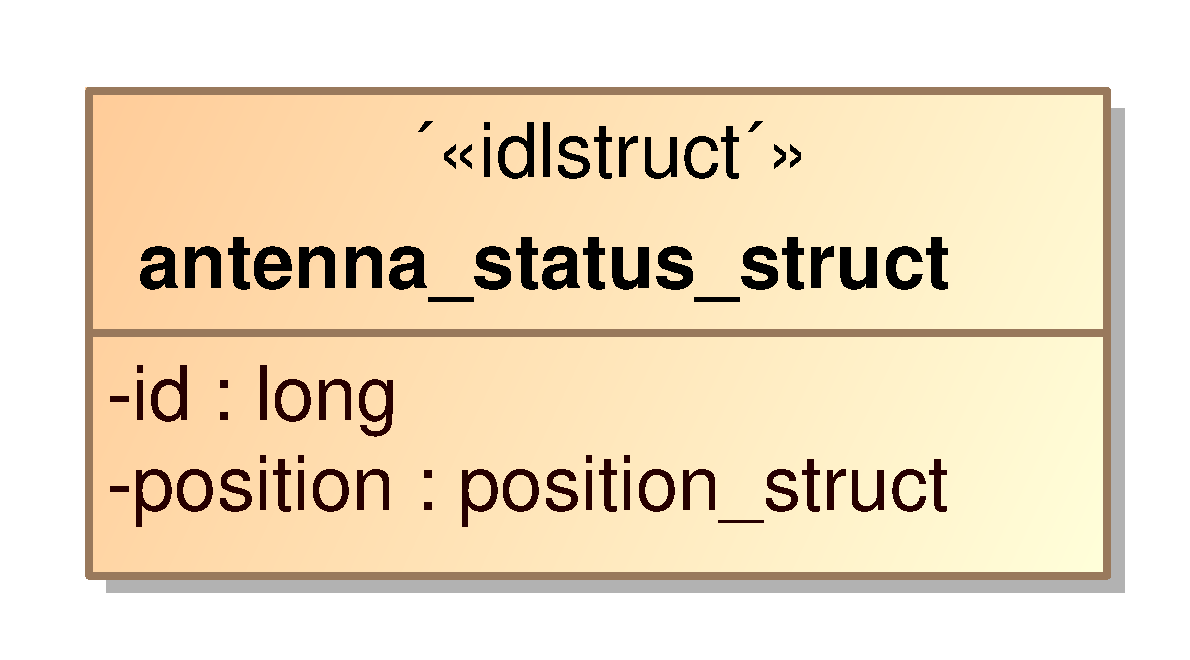
\includegraphics[scale=0.2]{images/idlstructb}
\caption{\label{fig:vs_diag}IDL Struct Definition}
\end{center}
\end{figure*} 

The code generated for that struct is defined in a common IDL interface, this
IDL file has the name of the project, in this case \verb+example1Common.idl+,
an example of the code generated:

\begin{center}
\begin{verbatim}
#ifndef example3_IDL
#define example3_IDL
#pragma prefix "alma"

module example3
{
    struct position_struct {
        long x;
        long y;
    };
    typedef sequence<position_struct> position_struct_seq;
	
    struct antenna_status_struct {
        long id;
        position_struct position;
    };
    typedef sequence<antenna_status_struct> antenna_status_struct_seq;
};
#endif //example3_IDL
\end{verbatim}
\end{center}

The code above also implement a  \verb+position_struct+ which is used by
\verb+antenna_status_struct+.

\subsubsection{Enumerations Definition}

The enumerations are defined as a class with the  \verb+<<enumeration>>+
stereotype in the model. The code for the enumerations is generated in the IDL
common file, t, in this case \verb+example1Common.idl+.

\begin{figure*}[h!t]
\begin{center}
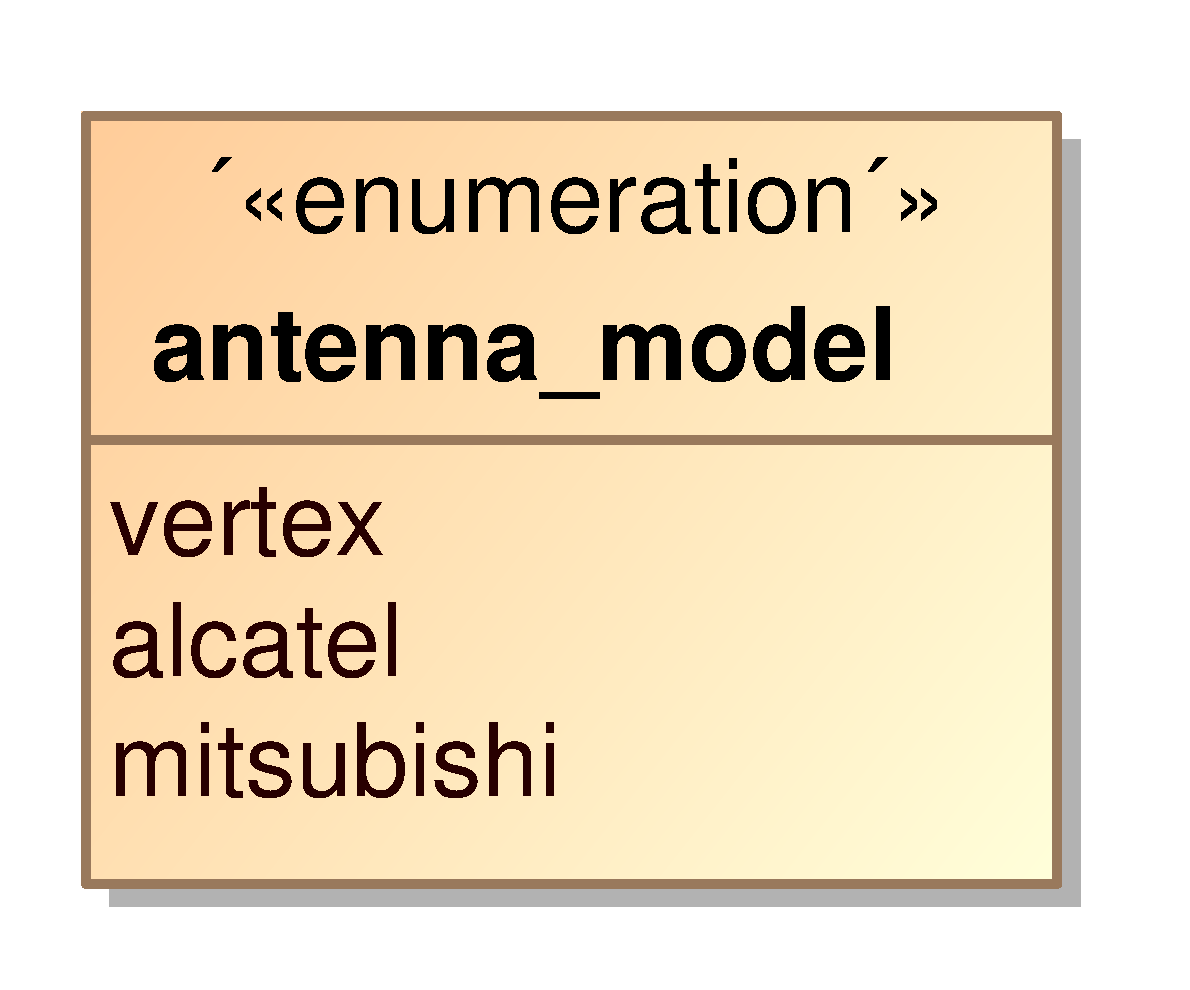
\includegraphics[scale=0.2]{images/enumeration}
\caption{\label{fig:vs_diag}Basic Enumeration Definition}
\end{center}
\end{figure*} 

An example of the code generated:

\begin{center}
\begin{verbatim}
....
module example3
{
    enum antenna_model { vertex, alcatel, mitsubishi };
....
\end{verbatim}
\end{center}

\subsubsection{Code Generated}

For convention, the model name has to be in a reverse domain name syntax,
(see the examples) i.e.:
\begin{center}
\begin{verbatim}
cl.alma.acsccg.example1
\end{verbatim}
\end{center}
The generator will generate the source code using the reverse domain name
syntax for generate the Java code. An example of the code generated for the
Figure 5 with the model name as \verb+cl.alma.acsccg.example1+ (this can be viewed in the folder structure).
\begin{center}
\begin{verbatim}
example3/
|-- idl
|   |-- BasicAntennaBase.idl
|   `-- example1Common.idl
|-- src
|   |-- cl
|   |   `-- alma
|   |       `-- acsccg
|   |           `-- example1
|   |               |-- BasicAntennaBaseHelper.java
|   |               `-- BasicAntennaBase.java
|   `-- Makefile
`-- test
    `-- CDB
        `-- MACI
            |-- Components
            |   `-- Components.xml
            |-- Containers
            	|-- javaContainer
            |   |   `-- javaContainer.xml
            |   `-- frodoContainer
            |       `-- frodoContainer.xml
            `-- Managers
                `-- Manager
                    `-- Manager.xml
\end{verbatim}
\end{center}

Also is generated the project Makefile, in which is defined the name of
the Jar file and the IDL interfaces to compile. The name of the Jar file is the last
name in the model name.

\newpage

\subsection{Java Interfaces}
The generator was designed to support Java interfaces in the UML model, this
interfaces are implemented by the generator writing the methods in the
component generated code.\\ 
\begin{figure*}[h!t]
\begin{center}
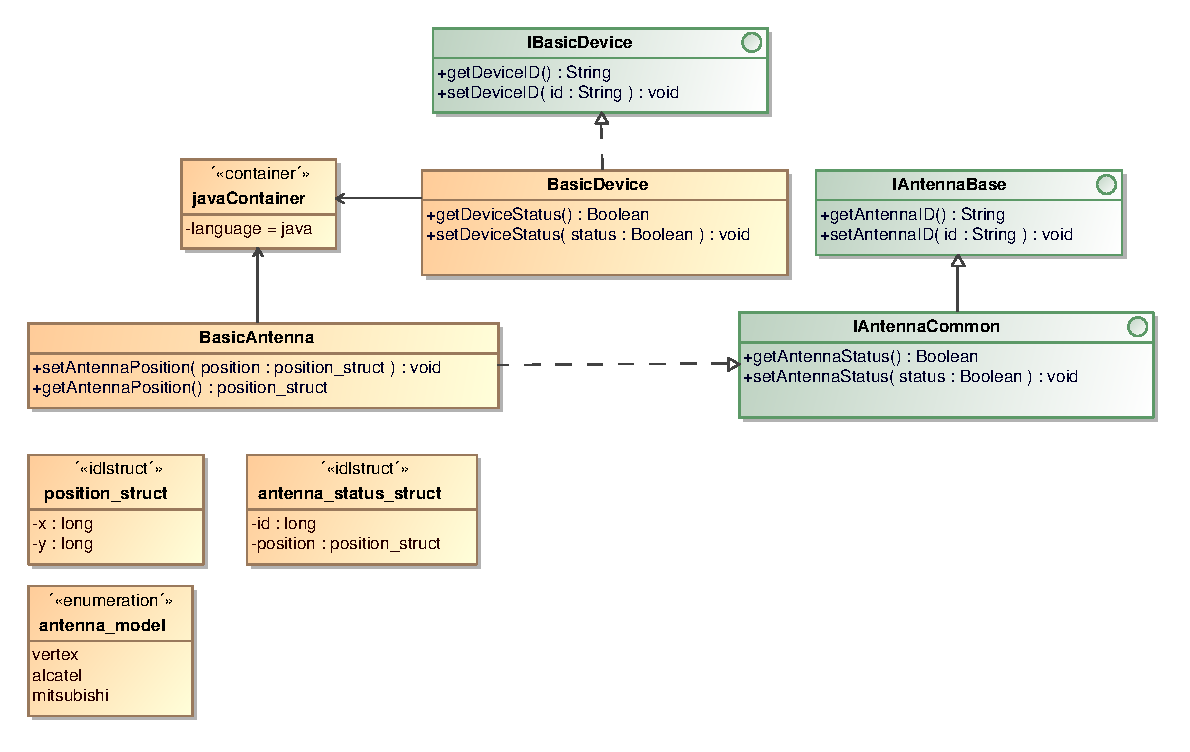
\includegraphics[scale=0.8]{images/example3}
\caption{\label{fig:vs_diag}Interfaces.}
\end{center}
\end{figure*}
\\
In the figure above, the class  \verb+BasicAntenna+ implements the Interface
\verb+IAntennaCommon+ and \verb+IAntennaCommon+ is extended from
\verb+IAntennaBase+, the generator also can implement the inheritance in
Interfaces. The code generated for the \verb+BasicAntenna+ component implements
the all the methods of all  implemented interfaces, if the interface is extended
in one or multiple levels, the generator implements all methods of the interface
inheritance (Java OOP constraints) and the IDL file implement this methods to.

Code generated, the component implementes the java interface defined in the
model above.
\begin{center}
\begin{verbatim}
...
public class BasicAntennaBase
      implements
         ComponentLifecycle,
              BasicAntennaBaseOperations,
              IAntennaCommon {
...
\end{verbatim}
\end{center}

And all methods from \verb+IAntennaCommon+, \verb+IAntennaBase+  are implemented
in the component.
\begin{center}
\begin{verbatim}
...
    /*
     * Implements the Interface methods.
     */
    @Override
    public boolean getAntennaStatus() {...

    @Override
    public void setAntennaStatus(boolean status) {...

    @Override
    public String getAntennaID() {...

    @Override
    public void setAntennaID(String id) {....
 ...
\end{verbatim}
\end{center}

Also the IDL file of the component is implemented with this methods to:
\begin{center}
\begin{verbatim}
...
#ifndef BasicAntenna_IDL
#define BasicAntenna_IDL
#include <acscomponent.idl>
#include <example3Common.idl>

#pragma prefix "alma"

module example3
{
    interface BasicAntennaBase : ACS::ACSComponent
    {
        void setAntennaPosition(in position_struct position);
        position_struct getAntennaPosition();
        boolean getAntennaStatus();
        void setAntennaStatus(in boolean status);
        string getAntennaID();
        void setAntennaID(in string id);
    };
};
#endif /* example3_IDL */
...
\end{verbatim}
\end{center}

This example can be downloaded from:
http://acsccg.googlecode.com/files/example3.tar.gz

\subsection{Inheritance}

\subsubsection{Multiple Level}
The generator is designed to support inheritance in one ore more inherited
levels, with the ability to override the inherited methods from the parenet, or,
override all methods inherited in all inherited levels.\\
This can be viewed in figure 11.

\begin{figure*}[h!t]
\begin{center}
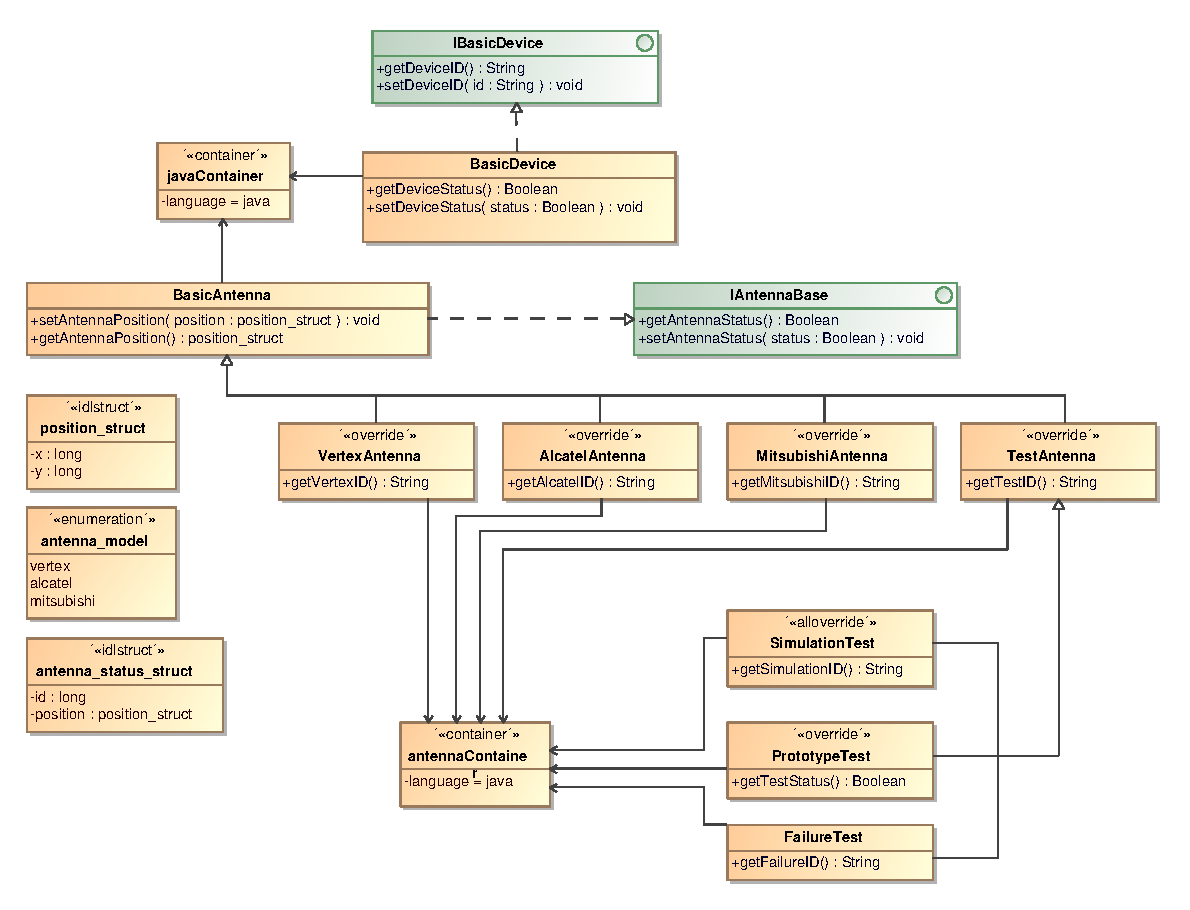
\includegraphics[scale=0.88]{images/example4}
\caption{\label{fig:vs_diag}Inheritance in the generator}
\end{center}
\end{figure*}

This example can be downloaded from:
http://acsccg.googlecode.com/files/example4.tar.gz

In the example above the classes with the  \verb+<<override>>+ stereotype will
override the methods from his parents in the Java generated code, and the
classes with the  \verb+<<alloverride>>+ will override all methods inherited in all
leves, i.e.: the class  \verb+SimulationTest+ will have his own methods, the 
\verb+TestAntenna+ methods, the  \verb+BasicAntenna+ methods (with the methods
of the implemented interface  \verb+IAntennaBase+).\\
If the component class has a parent class, the  \verb+initialize+ method of the
component will call the  \verb+initialize+ method of the parent class, an
example of this is:
\begin{center}
\begin{verbatim}
...
public class VertexAntennaBase extends BasicAntennaBase...

public void initialize(ContainerServices containerServices) {

		m_containerServices = containerServices;

		super.initialize(containerServices);
...
\end{verbatim}
\end{center}
The IDL files also implement the inheritance, an example of this:
\begin{center}
\begin{verbatim}
...
module example4
{
     interface AlcatelAntennaBase : BasicAntennaBase  
    {
        string getAlcatelID();
        void setAntennaPosition(in position_struct position);
        position_struct getAntennaPosition();
...
\end{verbatim}
\end{center}

Also if the class component is not inherited from other component or other
class, the IDL interface is extended from \verb+ACS::ACSComponent+, the
AlcatelAntennaBase is extended from BasicAntennaBase.

\subsection{Characteristic Component}
A class with the stereotype \verb+<<Characteristic>>+, if is extended from
other class, the generator will not implement the inheritance in the Java code,
because the Java OOP paradigm not support multiple inheritance (parallel
inheritance) and the class with \verb+<<Characteristic>>+, the generator will
generate the class already extended from ACS class
`CharacteristicComponentImpl`, also is generated the schema configuration .

\subsection{Notification Channel} 
 
 The ACS Notification Channel also is supported in the UML model.
 
 \begin{figure*}[h!t]
\begin{center}
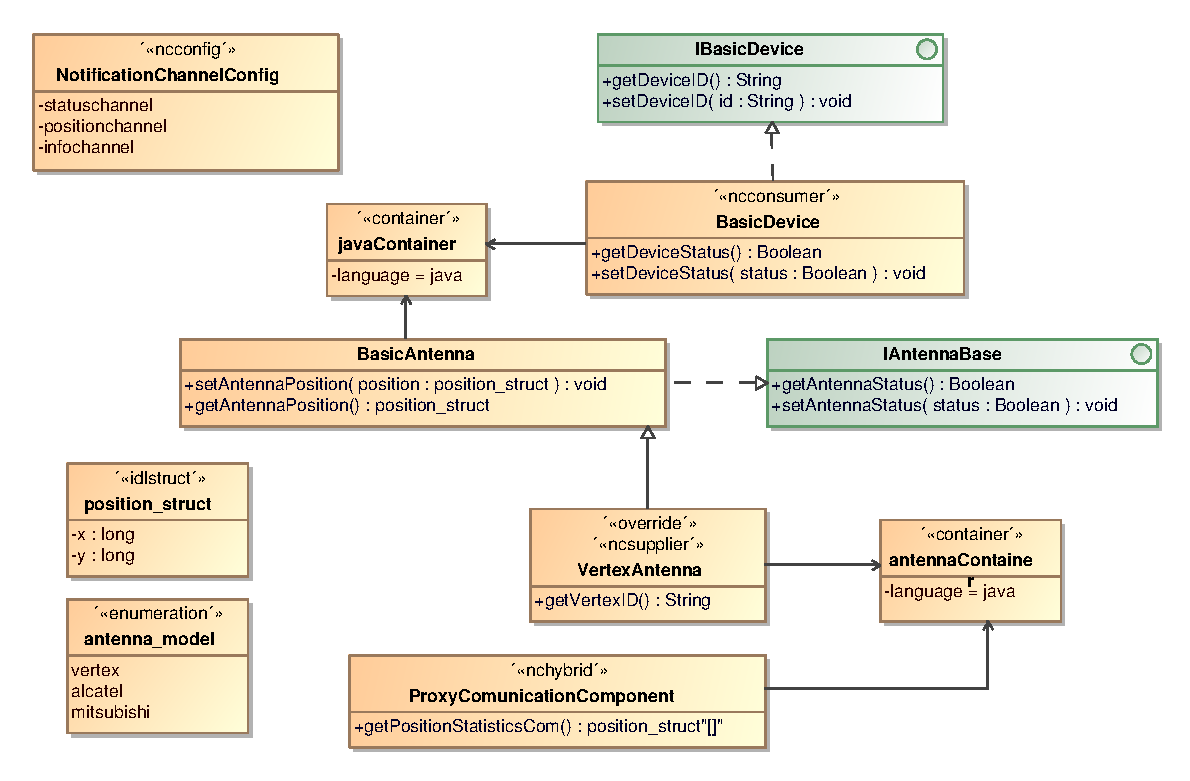
\includegraphics[scale=0.88]{images/example6}
\caption{\label{fig:vs_diag}Inheritance in the generator}
\end{center}
\end{figure*}
 
This example can be downloaded from:
http://acsccg.googlecode.com/files/example6.tar.gz\\
\\
In the example above exists a class with the \verb+<<ncconfig>>+ stereotype,
this class define the channels to use in the project, in the example they are
defined three channels \verb+statuschannel+, \verb+positionchannel+ and
\verb+infochannel+ generated in the common IDL interface, in this case
\verb+example6Common.idl+ , should only be one class with this stereotype.
\\
Also when this class is defined in the model, the generator define a common or
default channel called in this case \verb+defaultexample6channel+, the
\verb+example6+ in the channel name, is from the reverse domain name syntax on
model naming and a IDL struct for test the channel implementation, this struct
is called \verb+testMessageBlockEvent+, an example of the code generated :

\begin{center}
\begin{verbatim}
...
//Channels
const string CHANNELNAME_DEFAULTEXAMPLE6CHANNEL = "defaultexample6channel";
const string CHANNELNAME_STATUSCHANNEL = "statuschannel";
const string CHANNELNAME_POSITIONCHANNEL = "positionchannel";
const string CHANNELNAME_INFOCHANNEL = "infochannel";

 //Test Struct Event for the notification channels
struct testMessageBlockEvent
{
     double randomID;  
     string message;
 };
  typedef sequence<testMessageBlockEvent> testMessageBlockEvent_seq;
...
\end{verbatim}
\end{center}

Also in the example, they are classes with the \verb+<<ncsupplier>>+,
\verb+<<ncconsumer>>+ and the \verb+<<nchybrid>>+:

\subsubsection{ncsupplier}
The classes with  \verb+<<ncsupplier>>+ stereotype, will supply events in the
default channel defined by the generator, in this case the channel is called:\\
\verb+const string CHANNELNAME_DEFAULTEXAMPLE6CHANNEL="defaultexample6channel";+
Also the generator will implement the necessary methods to supply events ( a
default event called \verb+testMessageBlockEvent+) in the channel, an
example of the code generated:

\begin{center}
\begin{verbatim}
...

import alma.acs.nc.SimpleSupplier;
import alma.example6.testMessageBlockEvent;

...

    public void initialize(ContainerServices containerServices) {

        m_containerServices = containerServices;

        super.initialize(containerServices);

        m_logger = m_containerServices.getLogger();
        m_logger.info("initialize() called...");

        try {
            // Instantiate our supplier
                m_supplier = new SimpleSupplier(
                    alma.example6.CHANNELNAME_DEFAULTEXAMPLE6CHANNEL.value,
                m_containerServices);
        } catch (Exception e) {
            //throw new ComponentLifecycleException("failed to create
        SimpleSupplier for channel " + 
        alma.example6.CHANNELNAME_DEFAULTEXAMPLE6CHANNEL.value, e); 
        }

....

    public void sendEvents() throws CouldntPerformActionEx {
       m_logger.info("Now sending  testMessageBlockEvent events...");
        try {
            testMessageBlockEvent event = new testMessageBlockEvent(Math
                .random(), "Event");
            m_supplier.publishEvent(event);
        } catch (Throwable thr) {
            m_logger
                .log(Level.WARNING,
                    "failed to send testMessageBlockEvent. Will not try
                    again."); throw (new AcsJCouldntPerformActionEx(thr))
                    .toCouldntPerformActionEx();
        }
    }
\end{verbatim}
\end{center}

\subsubsection{ncconsumer}
The classes with  \verb+<<ncconsumer>>+ stereotype, will consume events in the
default channel defined by the generator, in this case the channel is called:\\
\verb+const string CHANNELNAME_DEFAULTEXAMPLE6CHANNEL="defaultexample6channel";+
Also the generator will implement the necessary methods to consume events ( a
default event called \verb+testMessageBlockEvent+) in the channel, an
example of the code generated:

\begin{center}
\begin{verbatim}
...
    private Consumer m_consumer;
    ....
        try {
            m_consumer = new Consumer(
                alma.example6.CHANNELNAME_DEFAULTEXAMPLE6CHANNEL.value,
                    m_containerServices);
                //Subscribe to a domain and event type.
            m_consumer.addSubscription(
                alma.example6.testMessageBlockEvent.class, this);
                m_consumer.consumerReady();
                m_logger
                    .info(" BasicDevice  is waiting for 
                    'testMessageBlockEvent'events."); 
                    } catch (Exception e) {
                if (m_consumer != null) {
            m_consumer.disconnect();
			           }
            /*
             if uncomment the next line, add  throws
             ComponentLifecycleException, but first check if is 
             inhitered class, can not be override the method. 
             the generator put the right code. */ 
             throw new ComponentLifecycleException( 
             "failed to connect as an event consumer to channel " +
             alma.example6.CHANNELNAME_DEFAULTEXAMPLE6CHANNEL.value); 
             }
    ....
    
...
\end{verbatim}
\end{center}


\subsubsection {nchybrid}
The classes with  \verb+<<nchybrid>>+ will consume and supply events in the
default channel defined by the generator, this class will implement the supply
and consume methods, variables and librarys to test the component. This methods
and variables are the same of the examples above.\\
\\
For the three stereotypes, if the components has not a parent class, the
generator will implement an ACS throw exception in the   \verb+initialize+
method of the component.

%\subsubsection{Abstract Classes}
%Same as interface implementation, the generator support the abstract class
%definition and generate the code.\\
%Classes with the \verb+<<Characteristic>>+ stereotype, the generator will no
%generate this classes as Abstract.

\subsection{Implemented Code vs Generated Code}
In every model driven development and code generators, is important how make a
strategy to separate the code already generated with the code implemented over
the generated code.\\
They are three ways solve this.

\subsubsection{EMF Veto Strategy and Inheritance}
The Veto EMF strategy (see Generator Optimization section) is a good solution
using inheritance to implement new things, but, must be create a new class for every change in our code to void
override the whole code already generated, so, this is not the best solution,
but, it works.

\subsubsection{GAP Desing Pattern}
The generation GAP desing pattern provides separate the code with all
hand-modifications implemented in sub-classes, this mean that the core classes
are generated only once and the hand-made implementations, are extended as
subclases from core classes.

\subsubsection{Protected Areas}
Xpand, provides protected areas to our generated code, this mean, that certain
areas with the protected tag with a unique autegenerated ID, can be modified by
the developer without loosing the hand-modifications over the generated code
when the code is re-generated (even if classes are changed in the model).
i.e.: This code went generated with protected areas.
\begin{verbatim}
1. public void getSimulationList() {
2. /*PROTECTED REGION ID(getSimulationList) ENABLED START*/
3.    //Implementation Method here!
4. /*PROTECTED REGION END*/
5. }

1. Method definition
2. Start Protected Area
3. Method hand implementation
4. End Protected Area
\end{verbatim}
Protected areas are specified in generator templates, the generator analize the
generated code, check the code with the template, and protect the area from the
regeneration. If the protected region is not in the templates, the generator
will void the area.\\
In methods, only the implementation is protected and for the code that scape
from UML model every class has a protected area for custom imports, variables and methods.

In every component generated exists three protected regions by default:\\
\\
A protected regions for custom imports:
\begin{verbatim}
/*PROTECTED REGION ID(VertexAntenna.ProtectedImports) ENABLED START*/
/* (non-javadoc!)
 * Autogenerated protected region, the imports in this protected area
 * are not generated, it's reserved to special features that they can't be
 * specified in the UML model
 */
/*PROTECTED REGION END*/
\end{verbatim}

A protected regions for custom variables definition:
\begin{verbatim}
/*PROTECTED REGION ID(VertexAntenna.ProtectedAttributes) ENABLED START*/
/* (non-javadoc!)
 * Autogenerated protected region, the imports in this protected area
 * are not generated, it's reserved for special features that they can't be
 * specified in the UML model
 */
/*PROTECTED REGION END*/
\end{verbatim}

A protected regions for custom variables initialization inside of initialize
method:
\begin{verbatim}
/*PROTECTED REGION ID(VertexAntenna.ProtectedAttributes) ENABLED START*/
/* (non-javadoc!)
 * Autogenerated protected region, the imports in this protected area
 * are not generated, it's reserved for special features that they can't be
 * specified in the UML model
 */
/*PROTECTED REGION END*/
\end{verbatim}

A protected regions for custom variables initialization inside of initialize
method:
\begin{verbatim}
/*PROTECTED REGION ID(VertexAntenna.ProtectedRegion) ENABLED START*/
/* (non-javadoc!)
 * Autogenerated protected region, the implementations in this protected area
 * are not generated, it's reserved to special features that they can't be
 * specified in the UML model
 */
/*PROTECTED REGION END*/
\end{verbatim}



